\documentclass{article}

\usepackage[final]{neurips_2024}



\usepackage[utf8]{inputenc} % allow utf-8 input
\usepackage[T1]{fontenc}    % use 8-bit T1 fonts
\usepackage{hyperref}       % hyperlinks
\usepackage{url}            % simple URL typesetting
\usepackage{booktabs}       % professional-quality tables
\usepackage{amsfonts}       % blackboard math symbols
\usepackage{nicefrac}       % compact symbols for 1/2, etc.
\usepackage{microtype}      % microtypography
\usepackage{xcolor}         % colors
\usepackage{amsmath}
\usepackage{graphicx}
\usepackage{pythonhighlight}
\usepackage{subcaption}
\usepackage{float}

\newcommand{\todo}[1]{\textcolor{red}{#1}}

\newcommand{\R}{\mathbb{R}}
\newcommand\Tstrut{\rule{0pt}{2.6ex}}

\title{Efficient Attention}


\author{
  Sahil Chaudhary \\
  \And
  Mrigank Pawagi \\
  \And
  Rohit Jorige \\
  \And
  Jajapuram Nagasai \\
  % \And
  % Bachelor of Technology \\
  % Indian Institute of Science\\
  % \texttt{\{sahilc, mrigankp, rohitrj, nagasaij\}@iisc.ac.in}
}

\begin{document}


\maketitle


\begin{abstract}
   % \todo{(1) Introduce transformers. (2) Talk about time complexity and why linformer. (3) Introduce fine-tuning and need for LoRA. (4) Mention contributions (experiments)} \\ 

    The transformer architecture revolutionized sequence transduction with its novel ``Scaled Dot-Product Attention'' by outperforming previous recurrent and convolutional models, while dispensing recurrence and convolutions entirely. However, these transformers are prohibitively slow for very long sequences due to their $\mathcal{O}(N^2)$ time complexity in the forward pass, where $N$ is the sequence length. By expressing the self-attention in these transformers as a linear dot-product of kernel feature maps and making use of the associativity property of matrix products can reduce the complexity to $\mathcal{O}(N)$. In addition to these theoritical results, recent empirical results suggest that training of and inference from these models can be made faster and more scalable. One such technique, `Low-Rank Adaption' or LoRA has proven to be particularly valuable in the scalable adaptation of pre-trained models to new tasks through fine-tuning. In this article, we will discuss the results mentioned above. Besides reproducing some of the experiments in these papers, our contributions include new experiments to explore these results. 
\end{abstract}



\section{Attention Architecture}
    The self-attention mechanism makes it possible to capture dependencies between different positions in a sequence by simultaneously attending to all positions. The ``Scaled Dot-Product Attention'' proposed by Vaswani et al.~\cite{vaswaniAttention} for an input sequence $x \in \R^{N \times F}$ is computed as $\text{Attention}(x) = \text{softmax}(QK^T/\sqrt{D})V$
    where $Q = xW_Q$ (queries), $K = xW_K$ (keys) and $V = xW_V$ (values). Note that $W_Q, W_K \in \R^{F \times D}$ and $W_V \in \R^{F \times M}$ are learned weights. Then the attention vector for the $i$-th position is given by the $i$-th row,
    \begin{align*}
        \text{Attention}(x)_i &= \text{softmax}\left(\frac{(QK^T)_i}{\sqrt{D}} \right) V = \frac{\sum_{j=1}^N \exp(Q_i^TK_j/\sqrt{D})V_j}{\sum_{j=1}^N \exp(Q_i^TK_j/\sqrt{D})} 
    \end{align*}
    Since $\exp(Q_i K_j^T / \sqrt{D})$ has to be determined and stored for every $i, j \in \{1, \ldots, N\}$, this leads to $\mathcal{O}(N^2)$ time and memory complexity~\footnote{More precisely, the complexity is $\mathcal{O}(N^2\max\{D, M\})$.}.

    \section{Towards Efficient Attention -- Linearized Attention}
    The exponential similarity function above can be replaced with any map $\text{sim}: \R^D \times \R^D \to \R_+$. This includes all kernels between the two spaces. Katharopoulos et al.~\cite{transformersRNN} show that given such a kernel with a feature representation $\phi$, we can rewrite the attention computation as
    \begin{align*}
        \text{Attention}(x)_i &= \frac{\sum_{j=1}^N \phi(Q_i)^T\phi(K_j)V_j}{\sum_{j=1}^N \phi(Q_i)^T\phi(K_j)} = \frac{\phi(Q_i)^T\sum_{j=1}^N \phi(K_j)V_j^T}{ \phi(Q_i)^T \sum_{j=1}^N \phi(K_j)}
    \end{align*}
    Since $\sum_{j=1}^N \phi(K_j)V_j^T$ and $\sum_{j=1}^N \phi(K_j)$ can be computed once reused for every query, this formulation has $\mathcal{O}(N)$ time and memory complexity~\footnote{More precisely, the complexity is $\mathcal{O}(NCM)$ where $C$ is the dimension of the range space of the feature map.}. 

\subsection{Transofrmers are RNNs}
The transformer architecture can further be used to efficiently train autoregressive models by masking the attention computation such that a position cannot be influenced by the subsequent positions. Then the attention for the $i$-th position can we written as given below. Note that we define $S_i = \sum_{j=1}^i \phi(K_j)V_j^T$ and $Z_i = \sum_{j=1}^i \phi(K_j)$. 
\begin{align*}
    \text{Attention}(x)_i &= \frac{\phi(Q_i)^T\sum_{j=1}^i \phi(K_j)V_j^T}{ \phi(Q_i)^T \sum_{j=1}^i \phi(K_j)} = \frac{\phi(Q_i)^TS_i}{\phi(Q_i)^TZ_i}
\end{align*}

Note that, $S_k$ and $Z_k$ can be computed from $S_{k-1}$ and $Z_{k-1}$ in constant time. This enables the transformer to be formulated as an RNN using the following recurrence relations. We set $s_0 = 0$ and $z_0 = 0$, and for all $k \ge 1$,
\begin{align*}
    s_k &= s_{k-1} + \phi(K_k)V_k^T = s_{k-1} + \phi(x_kW_K)(x_kW_V)^T \\
    z_k &= z_{k-1} + \phi(K_k) = z_{k-1} + \phi(x_kW_K)
\end{align*}
The resulting RNN thus has two hidden states -- the attention memory $s$ and the normalizer memory $z$. Then the output for the $i$-th transformer layer is given by
\begin{align*}
    T_i(x)=f_i \left( \left[ \frac{\phi(x_kW_Q)^Ts_k}{\phi(x_kW_Q)^Tz_k} + x_k \right]_{k=1}^N \right)
\end{align*}

\subsection{Experiments}
\subsubsection{Performance on random sequences}

To test the claim made for time complexity, we experimented on various length of random sequences for forward pass and backward pass in both of the models. We also experimented with the time taken to measure the attention in each of the case on random sequences.
\begin{center}
    \begin{tabular}{c c}
         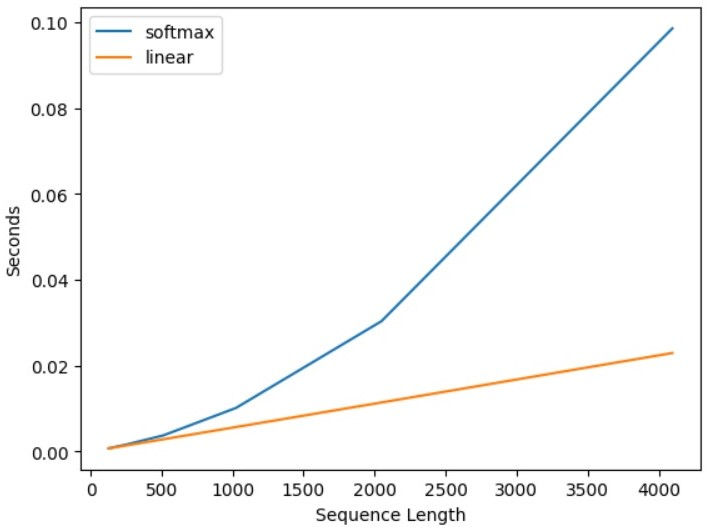
\includegraphics[width=0.2\textwidth]{images/forwardpassandbackwardpass.jpg} &
         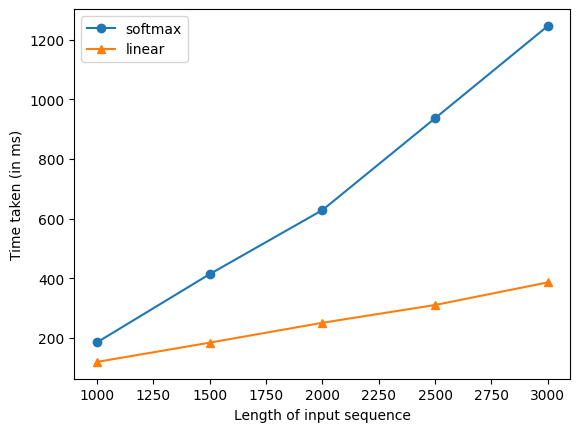
\includegraphics[width=0.2\textwidth]{images/attentiontimemeasure.png}\\
         Time taken for forward and backward pass vs sequential length & Time taken for attention measure vs sequential length
    \end{tabular}
\end{center}
\subsubsection{Occluded Image Completion}
We experimented the linear transformer over image generation tasks. We evaluate the model on image generation with autoregressive transformers on the widely used MNIST dataset. The architecture for this experiment is same to Katharopoulos et. al. Thanks to Katharaopoulos et. al., we had pretrained model for MNIST. We test the model on random image generation and measured the time, image completion task and quality measurement and time difference. 
\begin{center}
    \begin{tabular}{c c c }
        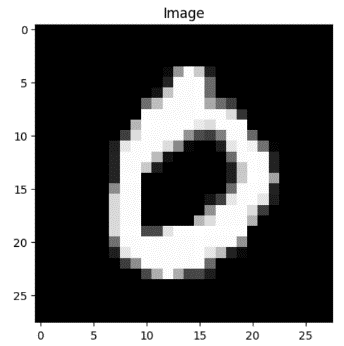
\includegraphics[width=0.1\textwidth]{images/input0.png} & 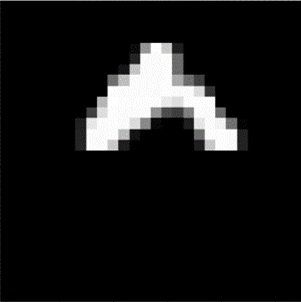
\includegraphics[width=0.1\textwidth]{images/occuluded0.png} & 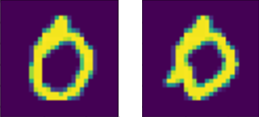
\includegraphics[width=0.2\textwidth]{images/result0.png} \\
		MNIST & Occuluded MNIST & Output
    \end{tabular}
\end{center}
    {Linear model was able to achieve faster and better image completion for given occluded input in comprasion to softmax based transformer}

\begin{center}
    \begin{tabular}{c|c|c|c}
        S.N & Number of Images generated & Linear & Softmax \\
        \hline
         1 & 100 & 33.45 s & 367.91 s \Tstrut\\
         2 & 200 & 67.46 s & 811.99 s\\
         3 & 300 & 76.46 s & 1248.15 s\\
    
    \end{tabular}
\end{center}

\label{gen_inst}


\section{Low-Rank Adaptation (LoRA) of Large Language Models}
Due to the compute requirements of large-scale pre-training of Large Language Models (LLMs), fine-tuning is a widely adopted paradigm for adapting models pre-trained on general domain data to particular tasks or domains. However, the large number of parameters in such models can make even fine-tuning prohibitively expensive. Work from Li et al.~\cite{li2018measuring} and Aghajanyan et al.~\cite{aghajanyan2020intrinsic} has demonstrated that models may be over-parameterized and may reside on a low intrinsic dimension. Taking inspiration from these results, Hu et al.~\cite{hu2022lora} showed empirically that the change in weights during model adaptation also has a low intrinsic rank. This not only makes it possible to achieve comparable accuracies with faster fine-tuning (due to fewer trainable parameters) but also makes it possible to easily switch different adaptators in and out during deployment. A matrix $M \in \R^{n \times m}$ can be rank decomposed as $M = UV$ where $U \in \R^{n \times r}$, $V \in \R^{r \times m}$ and $r$ is the rank of $M$. This reduces the number of trainable parameters from $mn$ to $r(n + m)$. Note that $r(n + m) \ll nm$ for small $r$. This decomposition of the update matrices during fine-tuning lies at the heart of LoRA. Note that $r$ is not known \textit{a priori} and one may have to try several small values of $r$.

\subsection{Experiments}
We train a base neural network on an image classification task on the MNIST dataset. Our base model was composed of three linear layers which together had 55.1K trainable parameters. This model has a test accuracy of approximately 93.2\%. We then created our variants of MNIST, namely Quantized MNIST, Rotated MNIST, and Inverted MNIST. These are illustrated below through an example.

\begin{center}
    \begin{tabular}{c c c c}
		
\includegraphics[width=0.1\textwidth]{images/normal_5.png} & 
\includegraphics[width=0.1\textwidth]{images/quantized_5.png} & 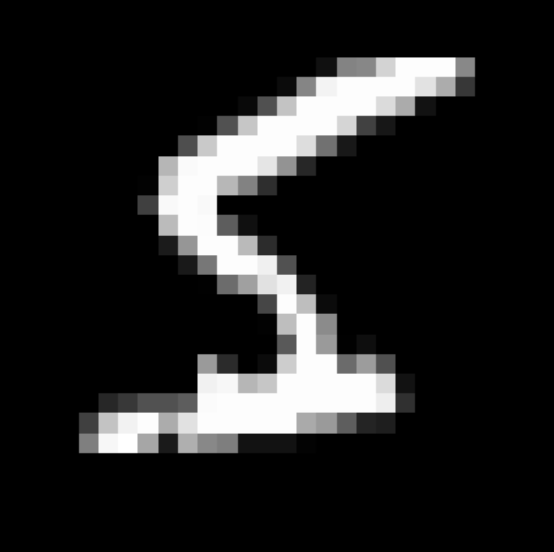
\includegraphics[width=0.1\textwidth]{images/rotated_5.png} & 
\includegraphics[width=0.1\textwidth]{images/inverted_5.png} \\
		MNIST & Quantized MNIST & Rotated MNIST & Inverted MNIST
    \end{tabular}
\end{center}

The accuracies of our base model on these modified datasets were approximately 85.58\%, 12.38\%, and 5.52\% respectively.


\subsubsection{Full Fine-Tuning}
We first fine-tuned our base model on the three datasets by modifying all 55.1K parameters. Our fine-tuned models achieved accuracies of approximately 93.57\%, 91.97\%, and 76.41\% on Quantized MNIST, Rotated MNIST, and Inverted MNIST respectively. These form our baselines for the fine-tuned models.

\subsubsection{Fine-Tuning with LoRA}
We then fine-tuned our base model on the three datasets using LoRA, with different values of $r$. We found that our fine-tuned models achieved accuracies comparable to their full fine-tuned counterparts with fewer trainable parameters. However due to the small size of our models, we could not observe any time improvements in training. The accuracies of our fine-tuned models in each domain and for each value of $r$ are given below.

\begin{center}
    \begin{tabular}{c | c | c | c | c}
        $r$ & Trainable Parameters & Quantized MNIST & Rotated MNIST & Inverted MNIST \\
        \hline
        % & & & & \\
        1 & 1.1K & 91.20\% & 37.53\% & 16.23\% \Tstrut \\
        2 & 2.1K & 91.30\% & 49.01\% & 17.92\% \\
        4 & 4.2K & 91.42\% & 69.10\% & 16.32\% \\
        8 & 8.4K & 91.39\% & 77.49\% & 32.19\% \\
        16 & 16.8K & 91.72\% & 86.95\% & 62.26\% \\
        32 & 33.6K & 92.31\% & 89.50\% & 68.06\% \\
        64 & 67.2K & 93.19\% & 90.41\% & 71.88\%
    \end{tabular}
\end{center}

\subsubsection{Full Training with LoRA}
We further explore whether LoRA can be used to train models from scratch, to observe if models have intrinsically low ranks. We trained separate models on each of our three modified MNIST datasets. The accuracies of these models are given below along with the respective $r$ values chosen.

\begin{center}
    \begin{tabular}{c | c | c | c | c}
        $r$ & Trainable Parameters & Quantized MNIST & Rotated MNIST & Inverted MNIST \\
        \hline
        % & & & & \\
        1 & 1.1K & 23.50\% & 25.91\% & 22.21\% \Tstrut \\
        2 & 2.1K & 37.48\% & 43.96\% & 45.81\% \\
        4 & 4.2K & 64.87\% & 62.60\% & 69.67\% \\
        8 & 8.4K & 77.96\% & 82.39\% & 83.11\% \\
        16 & 16.8K & 88.2\% & 86.76\% & 87.38\% \\
        32 & 33.6K & 90.13\% & 90.62\% & 90.25\% \\
        64 & 67.2K & 91.66\% & 91.85\% & 86.01\%
    \end{tabular}
\end{center}

\section{Acknowledgements}
We thank Dhruva Kashyap, one of the cockiest teaching assistants in UMC 203 and one of the last Emacs users, for his unwavering technical and emotional support throughout the preparation of this report. We are also extremely grateful to Chiranjib ki maa ka bhosada.

\bibliographystyle{plain} % We choose the "plain" reference style
\bibliography{cite} % Entries are in the refs.bib file

\end{document}
